
\documentclass[aspectratio=169,10pt]{beamer}

% ==================================================
% THEME AND PACKAGES
% ==================================================
\usetheme{Madrid}
\usecolortheme{seahorse}

\usepackage[T1]{fontenc}
\usepackage{lmodern}
\usepackage{xcolor}
\usepackage{listings}
\usepackage{tikz}
\usepackage{booktabs}
\usepackage{array}
\usepackage{amsmath}

\usetikzlibrary{
    arrows.meta,
    positioning,
    shapes.geometric
}

% ==================================================
% COLORS
% ==================================================
\definecolor{navy}{RGB}{20,55,105}
\definecolor{codebg}{RGB}{247,249,252}
\definecolor{codeblue}{RGB}{0,65,145}
\definecolor{codegreen}{RGB}{50,110,65}
\definecolor{codered}{RGB}{160,45,45}

\setbeamercolor{structure}{fg=navy}

% ==================================================
% CODE FORMATTING
% ==================================================
\lstdefinestyle{cstyle}{
    language=C,
    basicstyle=\ttfamily\tiny,
    keywordstyle=\color{codeblue}\bfseries,
    commentstyle=\color{codegreen},
    stringstyle=\color{codered},
    backgroundcolor=\color{codebg},
    frame=single,
    rulecolor=\color{gray!35},
    breaklines=true,
    showstringspaces=false,
    tabsize=4,
    numbers=left,
    numberstyle=\tiny\color{gray},
    numbersep=5pt,
    xleftmargin=0.25cm
}

\lstdefinestyle{terminal}{
    basicstyle=\ttfamily\scriptsize,
    backgroundcolor=\color{black!7},
    frame=single,
    breaklines=true
}

% ==================================================
% PRESENTATION INFORMATION
% ==================================================
\title[OS Lab: IPC]{Inter-Process Communication in Linux}
\subtitle{Weeks 6, 7 and 8\\
FIFO, Message Queues and Shared Memory}

\author{Dr. Siddhant Thapliyal}

\institute{
Department of Computer Science and Engineering\\
Graphic Era Deemed to be University
}

\date{Academic Session 2026--27}

% ==================================================
% DOCUMENT
% ==================================================
\begin{document}

% ==================================================
% SLIDE 1: TITLE
% ==================================================
\begin{frame}
\titlepage
\end{frame}

% ==================================================
% SLIDE 2: OBJECTIVES
% ==================================================
\begin{frame}{Learning Objectives}

By the end of these laboratory sessions, students
will be able to:

\begin{enumerate}
    \item Explain Inter-Process Communication (IPC).
    \item Implement FIFO-based communication.
    \item Implement System V message queues.
    \item Implement System V shared memory.
    \item Explain the system calls used in each mechanism.
    \item Execute sender and receiver programs
    in separate Linux terminals.
    \item Compare the three IPC mechanisms.
    \item Identify common IPC errors and
    resource-management requirements.
\end{enumerate}

\end{frame}

% ==================================================
% SLIDE 3: IPC INTRODUCTION
% ==================================================
\begin{frame}{Introduction to Inter-Process Communication}

\begin{block}{Definition}
Inter-Process Communication (IPC) allows
independent processes to exchange information
and coordinate their activities.
\end{block}

\begin{itemize}
    \item Processes normally have separate
    virtual address spaces.
    \item IPC provides controlled mechanisms
    for exchanging data.
    \item IPC is used in operating systems,
    servers, databases and distributed applications.
\end{itemize}

\begin{alertblock}{Examples}
FIFO, Message Queue, Shared Memory,
Semaphore, Pipe and Socket.
\end{alertblock}

\end{frame}

% ==================================================
% SLIDE 4: COMPARISON OVERVIEW
% ==================================================
\begin{frame}{IPC Mechanisms Covered}

\begin{center}
\begin{tabular}{p{3cm}p{3.8cm}p{4.5cm}}
\toprule
\textbf{Mechanism} &
\textbf{Communication Model} &
\textbf{Main System Calls}\\
\midrule
FIFO &
Named byte stream &
\texttt{mkfifo(), open(), read(), write()}\\
\addlinespace
Message Queue &
Message-oriented exchange &
\texttt{msgget(), msgsnd(), msgrcv()}\\
\addlinespace
Shared Memory &
Common memory segment &
\texttt{shmget(), shmat(), shmdt()}\\
\bottomrule
\end{tabular}
\end{center}

\end{frame}

% ==================================================
% WEEK 6
% ==================================================
\section{Week 6: FIFO / Named Pipe}

\begin{frame}
\centering
\vfill
{\Huge\bfseries WEEK 6}\\[0.5cm]
{\LARGE Implementation of FIFO / Named Pipe}\\[0.4cm]
{\large Inter-Process Communication}
\vfill
\end{frame}

% ==================================================
% SLIDE: FIFO AIM
% ==================================================
\begin{frame}{Week 6: Aim and Theory}

\begin{block}{Aim}
To implement communication between processes
using FIFO.
\end{block}

\begin{block}{Theory}
A FIFO is a named pipe. Unlike an unnamed pipe,
it can be used by unrelated processes.
\end{block}

\begin{itemize}
    \item FIFO stands for First In, First Out.
    \item It has a name in the filesystem.
    \item Data is read in the order it is written.
    \item It provides byte-stream communication.
    \item It is commonly used for communication
    between separate processes.
\end{itemize}

\end{frame}

% ==================================================
% SLIDE: FIFO SYSTEM CALLS
% ==================================================
\begin{frame}[fragile]{FIFO: Important System Calls}

\begin{block}{Creating a FIFO}
\begin{lstlisting}[style=cstyle]
mkfifo("myfifo", 0666);
\end{lstlisting}
\end{block}

\begin{center}
\begin{tabular}{ll}
\toprule
\textbf{Function} & \textbf{Purpose}\\
\midrule
\texttt{mkfifo()} & Create a named pipe\\
\texttt{open()} & Open the FIFO\\
\texttt{write()} & Send data\\
\texttt{read()} & Receive data\\
\texttt{close()} & Close descriptor\\
\texttt{unlink()} & Remove FIFO name\\
\bottomrule
\end{tabular}
\end{center}

\begin{alertblock}{Important}
The permission mode \texttt{0666} is subject
to the process's \texttt{umask}.
\end{alertblock}

\end{frame}

% ==================================================
% SLIDE: FIFO DIAGRAM
% ==================================================
\begin{frame}{FIFO: Communication Architecture}

\begin{center}
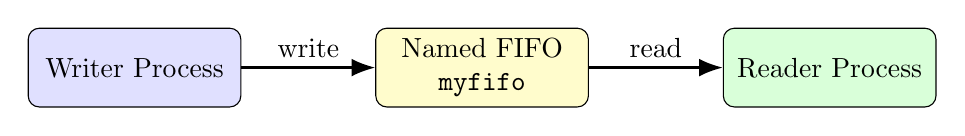
\begin{tikzpicture}[
    box/.style={
        draw,
        rounded corners,
        minimum width=2.7cm,
        minimum height=1cm,
        align=center
    }
]
\node[box,fill=blue!12] (writer)
    {Writer Process};

\node[box,fill=yellow!20,right=1.7cm of writer]
    (fifo) {Named FIFO\\\texttt{myfifo}};

\node[box,fill=green!15,right=1.7cm of fifo]
    (reader) {Reader Process};

\draw[-{Latex[length=3mm]},thick]
    (writer) -- node[above]{write} (fifo);

\draw[-{Latex[length=3mm]},thick]
    (fifo) -- node[above]{read} (reader);
\end{tikzpicture}
\end{center}

\vspace{0.5cm}

\begin{itemize}
    \item Writer opens FIFO using \texttt{O\_WRONLY}.
    \item Reader opens FIFO using \texttt{O\_RDONLY}.
    \item The kernel manages the FIFO's data buffer.
    \item The FIFO pathname identifies the channel.
\end{itemize}

\end{frame}

% ==================================================
% SLIDE: FIFO WRITER
% ==================================================
\begin{frame}[fragile]{Week 6: Writer Program}

\begin{lstlisting}[style=cstyle]
#include <stdio.h>
#include <stdlib.h>
#include <string.h>
#include <sys/stat.h>
#include <fcntl.h>
#include <unistd.h>

int main(void)
{
    int fd;
    char message[100];

    mkfifo("myfifo", 0666);

    fd = open("myfifo", O_WRONLY);

    if (fd == -1)
    {
        perror("open");
        return EXIT_FAILURE;
    }

    printf("Enter message: ");
    fgets(message, sizeof(message), stdin);

    write(fd, message, strlen(message) + 1);

    close(fd);

    return EXIT_SUCCESS;
}
\end{lstlisting}

\end{frame}

% ==================================================
% SLIDE: FIFO WRITER EXPLANATION
% ==================================================
\begin{frame}{Explanation: FIFO Writer}

\begin{enumerate}
    \item \texttt{mkfifo()} creates a named FIFO.
    \item \texttt{open()} opens it for writing.
    \item \texttt{fgets()} reads a message from the user.
    \item \texttt{write()} sends bytes through the FIFO.
    \item \texttt{close()} closes the write descriptor.
\end{enumerate}

\begin{alertblock}{Important Observation}
With normal blocking behavior, opening a FIFO
for writing generally waits until a reader
opens the FIFO.
\end{alertblock}

\end{frame}

% ==================================================
% SLIDE: FIFO READER
% ==================================================
\begin{frame}[fragile]{Week 6: Reader Program}

\begin{lstlisting}[style=cstyle]
#include <stdio.h>
#include <stdlib.h>
#include <fcntl.h>
#include <unistd.h>

int main(void)
{
    int fd;
    char buffer[100];

    fd = open("myfifo", O_RDONLY);

    if (fd == -1)
    {
        perror("open");
        return EXIT_FAILURE;
    }

    read(fd, buffer, sizeof(buffer));

    printf("Received: %s", buffer);

    close(fd);
    unlink("myfifo");

    return EXIT_SUCCESS;
}
\end{lstlisting}

\end{frame}

% ==================================================
% SLIDE: FIFO READER EXPLANATION
% ==================================================
\begin{frame}{Explanation: FIFO Reader}

\begin{enumerate}
    \item \texttt{open()} opens the FIFO for reading.
    \item \texttt{read()} receives bytes from the FIFO.
    \item Received data is stored in \texttt{buffer}.
    \item \texttt{printf()} displays the message.
    \item \texttt{close()} closes the descriptor.
    \item \texttt{unlink()} removes the FIFO pathname.
\end{enumerate}

\begin{block}{Programming Note}
Production code should check the return values
of \texttt{mkfifo()}, \texttt{read()} and
\texttt{write()}, and ensure that received text
is properly terminated before printing.
\end{block}

\end{frame}

% ==================================================
% SLIDE: FIFO EXECUTION
% ==================================================
\begin{frame}[fragile]{Week 6: Compilation and Execution}

Compile both programs:

\begin{lstlisting}[style=terminal]
gcc writer.c -o writer
gcc reader.c -o reader
\end{lstlisting}

\textbf{Terminal 1: Reader}

\begin{lstlisting}[style=terminal]
./reader
\end{lstlisting}

\textbf{Terminal 2: Writer}

\begin{lstlisting}[style=terminal]
./writer
Enter message: Hello Graphic Era
\end{lstlisting}

\textbf{Terminal 1 Output}

\begin{lstlisting}[style=terminal]
Received: Hello Graphic Era
\end{lstlisting}

\begin{block}{Result}
Inter-process communication using FIFO
was successfully demonstrated.
\end{block}

\end{frame}

% ==================================================
% SLIDE: FIFO DISCUSSION
% ==================================================
\begin{frame}{Week 6: Important Discussion Points}

\begin{enumerate}
    \item Why can unrelated processes use FIFO?
    \item Why must both programs use the same pathname?
    \item What happens if the reader starts before the writer?
    \item What happens if the writer starts before the reader?
    \item What is the purpose of \texttt{unlink()}?
    \item How is FIFO different from an unnamed pipe?
\end{enumerate}

\begin{alertblock}{Key Concept}
FIFO is named in the filesystem, but its
transferred data is handled through kernel buffers.
\end{alertblock}

\end{frame}

% ==================================================
% WEEK 7
% ==================================================
\section{Week 7: Message Queue}

\begin{frame}
\centering
\vfill
{\Huge\bfseries WEEK 7}\\[0.5cm]
{\LARGE Implementation of Message Queue}\\[0.4cm]
{\large System V Inter-Process Communication}
\vfill
\end{frame}

% ==================================================
% SLIDE: MQ AIM
% ==================================================
\begin{frame}{Week 7: Aim and Theory}

\begin{block}{Aim}
To implement Inter-Process Communication
using System V message queues.
\end{block}

\begin{block}{Theory}
A message queue allows processes to exchange
discrete messages through a kernel-managed queue.
\end{block}

\begin{itemize}
    \item Messages have a type.
    \item Messages can contain application data.
    \item Sender and receiver can be unrelated processes.
    \item The receiver can select messages by type.
    \item The queue remains until explicitly removed
    or otherwise cleaned up.
\end{itemize}

\end{frame}

% ==================================================
% SLIDE: MQ CALLS
% ==================================================
\begin{frame}{System V Message Queue Functions}

\begin{center}
\begin{tabular}{p{3cm}p{8cm}}
\toprule
\textbf{Function} & \textbf{Purpose}\\
\midrule
\texttt{ftok()} &
Generates a key from a filesystem path and project identifier.\\
\addlinespace
\texttt{msgget()} &
Creates or accesses a message queue.\\
\addlinespace
\texttt{msgsnd()} &
Sends a message to the queue.\\
\addlinespace
\texttt{msgrcv()} &
Receives a message from the queue.\\
\addlinespace
\texttt{msgctl()} &
Controls or removes the queue.\\
\bottomrule
\end{tabular}
\end{center}

\end{frame}

% ==================================================
% SLIDE: MQ ARCHITECTURE
% ==================================================
\begin{frame}{Message Queue Architecture}

\begin{center}
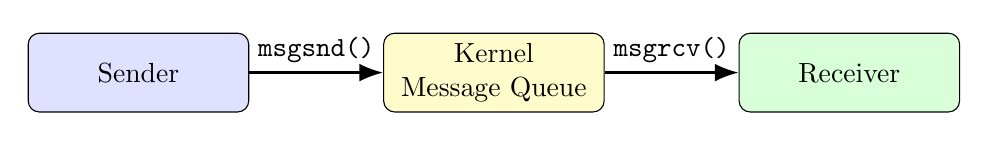
\begin{tikzpicture}[
box/.style={
    draw,
    rounded corners,
    minimum width=2.8cm,
    minimum height=1cm,
    align=center
}
]
\node[box,fill=blue!12] (sender)
    {Sender};

\node[box,fill=yellow!20,right=1.7cm of sender]
    (queue) {Kernel\\Message Queue};

\node[box,fill=green!15,right=1.7cm of queue]
    (receiver) {Receiver};

\draw[-{Latex[length=3mm]},thick]
(sender) -- node[above]{\texttt{msgsnd()}} (queue);

\draw[-{Latex[length=3mm]},thick]
(queue) -- node[above]{\texttt{msgrcv()}} (receiver);
\end{tikzpicture}
\end{center}

\vspace{0.4cm}

\begin{block}{Key Difference from FIFO}
A message queue preserves message boundaries,
whereas FIFO transfers a stream of bytes.
\end{block}

\end{frame}

% ==================================================
% SLIDE: MQ STRUCTURE
% ==================================================
\begin{frame}[fragile]{Message Structure}

The programs use the following structure:

\begin{lstlisting}[style=cstyle]
struct message
{
    long type;
    char text[100];
};
\end{lstlisting}

\begin{itemize}
    \item \texttt{type}: positive message type.
    \item \texttt{text}: message payload.
\end{itemize}

\begin{block}{Important}
The message size supplied to
\texttt{msgsnd()} and \texttt{msgrcv()}
does not include the \texttt{long type} field.
\end{block}

\end{frame}

% ==================================================
% SLIDE: MQ SENDER
% ==================================================
\begin{frame}[fragile]{Week 7: Sender Program}

\begin{lstlisting}[style=cstyle]
#include <stdio.h>
#include <stdlib.h>
#include <string.h>
#include <sys/ipc.h>
#include <sys/msg.h>

struct message
{
    long type;
    char text[100];
};

int main(void)
{
    key_t key;
    int msgid;
    struct message msg;

    key = ftok(".", 'A');

    msgid = msgget(key, 0666 | IPC_CREAT);

    if (msgid == -1)
    {
        perror("msgget");
        return EXIT_FAILURE;
    }

    msg.type = 1;

    printf("Enter message: ");
    fgets(msg.text, sizeof(msg.text), stdin);

    msgsnd(msgid, &msg,
           strlen(msg.text) + 1, 0);

    printf("Message sent.\n");

    return EXIT_SUCCESS;
}
\end{lstlisting}

\end{frame}

% ==================================================
% SLIDE: MQ SENDER EXPLANATION
% ==================================================
\begin{frame}{Explanation: Message Queue Sender}

\begin{enumerate}
    \item \texttt{ftok()} generates an IPC key.
    \item \texttt{msgget()} creates or accesses the queue.
    \item \texttt{msg.type = 1} assigns a message type.
    \item \texttt{fgets()} accepts input.
    \item \texttt{msgsnd()} sends the message.
\end{enumerate}

\begin{block}{Function Syntax}
\texttt{msgsnd(msgid, \&msg, size, flags);}
\end{block}

\begin{alertblock}{Important}
A successful \texttt{msgsnd()} normally queues
the message without requiring the receiver
to be running at that exact moment.
\end{alertblock}

\end{frame}

% ==================================================
% SLIDE: MQ RECEIVER
% ==================================================
\begin{frame}[fragile]{Week 7: Receiver Program}

\begin{lstlisting}[style=cstyle]
#include <stdio.h>
#include <stdlib.h>
#include <sys/ipc.h>
#include <sys/msg.h>

struct message
{
    long type;
    char text[100];
};

int main(void)
{
    key_t key;
    int msgid;
    struct message msg;

    key = ftok(".", 'A');

    msgid = msgget(key, 0666 | IPC_CREAT);

    if (msgid == -1)
    {
        perror("msgget");
        return EXIT_FAILURE;
    }

    msgrcv(msgid, &msg,
           sizeof(msg.text), 1, 0);

    printf("Received: %s", msg.text);

    msgctl(msgid, IPC_RMID, NULL);

    return EXIT_SUCCESS;
}
\end{lstlisting}

\end{frame}

% ==================================================
% SLIDE: MQ RECEIVER EXPLANATION
% ==================================================
\begin{frame}{Explanation: Message Queue Receiver}

\begin{enumerate}
    \item Generate the same IPC key.
    \item Access the same message queue.
    \item Receive a message of type \texttt{1}.
    \item Display the received message.
    \item Remove the queue using
    \texttt{msgctl(..., IPC\_RMID, ...)}.
\end{enumerate}

\begin{block}{Message Selection}
In this program, the message type argument
to \texttt{msgrcv()} is \texttt{1}.
\end{block}

\begin{alertblock}{Programming Note}
Check the return values of \texttt{ftok()},
\texttt{msgsnd()}, \texttt{msgrcv()} and
\texttt{msgctl()} in robust applications.
\end{alertblock}

\end{frame}

% ==================================================
% SLIDE: MQ EXECUTION
% ==================================================
\begin{frame}[fragile]{Week 7: Compilation and Execution}

\textbf{Compile:}

\begin{lstlisting}[style=terminal]
gcc sender.c -o sender
gcc receiver.c -o receiver
\end{lstlisting}

\textbf{Terminal 1: Sender}

\begin{lstlisting}[style=terminal]
./sender
Enter message: Welcome to OS Lab
Message sent.
\end{lstlisting}

\textbf{Terminal 2: Receiver}

\begin{lstlisting}[style=terminal]
./receiver
Received: Welcome to OS Lab
\end{lstlisting}

\begin{block}{Result}
Communication using System V message
queues was successfully implemented.
\end{block}

\end{frame}

% ==================================================
% SLIDE: MQ OBSERVATIONS
% ==================================================
\begin{frame}{Message Queue: Important Observations}

\begin{itemize}
    \item A message queue uses a kernel-managed
    identifier.
    \item Messages can be selected by type.
    \item The sender and receiver do not need
    a parent-child relationship.
    \item Messages are retained until received
    or the queue is removed.
    \item Queue capacity is finite.
\end{itemize}

\begin{block}{Useful Linux Commands}
\texttt{ipcs -q}: List System V message queues.

\texttt{ipcrm -q ID}: Remove a queue by ID.
\end{block}

\end{frame}

% ==================================================
% WEEK 8
% ==================================================
\section{Week 8: Shared Memory}

\begin{frame}
\centering
\vfill
{\Huge\bfseries WEEK 8}\\[0.5cm]
{\LARGE Implementation of Shared Memory}\\[0.4cm]
{\large System V Inter-Process Communication}
\vfill
\end{frame}

% ==================================================
% SLIDE: SHM AIM
% ==================================================
\begin{frame}{Week 8: Aim and Theory}

\begin{block}{Aim}
To implement Inter-Process Communication
using shared memory.
\end{block}

\begin{block}{Theory}
Shared memory enables multiple processes
to access a common memory segment.
\end{block}

\begin{itemize}
    \item Processes attach to the same shared segment.
    \item Data is accessed through memory operations.
    \item Processes can read and modify shared data.
    \item Explicit synchronization may be necessary
    for concurrent access.
\end{itemize}

\end{frame}

% ==================================================
% SLIDE: SHM CALLS
% ==================================================
\begin{frame}{Shared Memory: Important System Calls}

\begin{center}
\begin{tabular}{p{3cm}p{8cm}}
\toprule
\textbf{Function} & \textbf{Purpose}\\
\midrule
\texttt{ftok()} &
Generate an IPC key.\\
\addlinespace
\texttt{shmget()} &
Create or access a shared memory segment.\\
\addlinespace
\texttt{shmat()} &
Attach the segment to a process address space.\\
\addlinespace
\texttt{shmdt()} &
Detach the segment from a process.\\
\addlinespace
\texttt{shmctl()} &
Control or mark the segment for removal.\\
\bottomrule
\end{tabular}
\end{center}

\end{frame}

% ==================================================
% SLIDE: SHM ARCHITECTURE
% ==================================================
\begin{frame}{Shared Memory Architecture}

\begin{center}
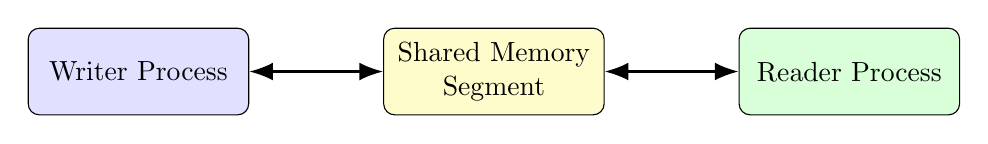
\begin{tikzpicture}[
box/.style={
    draw,
    rounded corners,
    minimum width=2.8cm,
    minimum height=1.1cm,
    align=center
}
]
\node[box,fill=blue!12] (writer)
    {Writer Process};

\node[box,fill=yellow!20,right=1.7cm of writer]
    (memory) {Shared Memory\\Segment};

\node[box,fill=green!15,right=1.7cm of memory]
    (reader) {Reader Process};

\draw[{Latex[length=3mm]}-{Latex[length=3mm]},thick]
(writer) -- (memory);

\draw[{Latex[length=3mm]}-{Latex[length=3mm]},thick]
(memory) -- (reader);
\end{tikzpicture}
\end{center}

\vspace{0.4cm}

\begin{alertblock}{Key Difference}
Unlike FIFO and message queues, shared memory
allows processes to access a common region
without sending each message through a
read/write IPC operation.
\end{alertblock}

\end{frame}

% ==================================================
% SLIDE: SHM WRITER
% ==================================================
\begin{frame}[fragile]{Week 8: Writer Program}

\begin{lstlisting}[style=cstyle]
#include <stdio.h>
#include <stdlib.h>
#include <string.h>
#include <sys/ipc.h>
#include <sys/shm.h>

int main(void)
{
    key_t key;
    int shmid;
    char *shared;

    key = ftok(".", 'S');

    shmid = shmget(key, 1024,
                   0666 | IPC_CREAT);

    if (shmid == -1)
    {
        perror("shmget");
        return EXIT_FAILURE;
    }

    shared = (char *)shmat(shmid, NULL, 0);

    if (shared == (char *)-1)
    {
        perror("shmat");
        return EXIT_FAILURE;
    }

    printf("Enter data: ");
    fgets(shared, 1024, stdin);

    printf("Data written to shared memory.\n");

    shmdt(shared);

    return EXIT_SUCCESS;
}
\end{lstlisting}

\end{frame}

% ==================================================
% SLIDE: SHM WRITER EXPLANATION
% ==================================================
\begin{frame}{Explanation: Shared Memory Writer}

\begin{enumerate}
    \item \texttt{ftok()} generates an IPC key.
    \item \texttt{shmget()} obtains a shared memory segment.
    \item \texttt{shmat()} attaches the segment.
    \item \texttt{fgets()} writes data into shared memory.
    \item \texttt{shmdt()} detaches the segment.
\end{enumerate}

\begin{block}{Important Observation}
The writer accesses shared memory through
a pointer returned by \texttt{shmat()}.
\end{block}

\end{frame}

% ==================================================
% SLIDE: SHM READER
% ==================================================
\begin{frame}[fragile]{Week 8: Reader Program}

\begin{lstlisting}[style=cstyle]
#include <stdio.h>
#include <stdlib.h>
#include <sys/ipc.h>
#include <sys/shm.h>

int main(void)
{
    key_t key;
    int shmid;
    char *shared;

    key = ftok(".", 'S');

    shmid = shmget(key, 1024, 0666);

    if (shmid == -1)
    {
        perror("shmget");
        return EXIT_FAILURE;
    }

    shared = (char *)shmat(shmid, NULL, 0);

    if (shared == (char *)-1)
    {
        perror("shmat");
        return EXIT_FAILURE;
    }

    printf("Data received: %s", shared);

    shmdt(shared);

    shmctl(shmid, IPC_RMID, NULL);

    return EXIT_SUCCESS;
}
\end{lstlisting}

\end{frame}

% ==================================================
% SLIDE: SHM READER EXPLANATION
% ==================================================
\begin{frame}{Explanation: Shared Memory Reader}

\begin{enumerate}
    \item Generate the same key.
    \item Locate the shared memory segment.
    \item Attach the segment using \texttt{shmat()}.
    \item Read data using the shared pointer.
    \item Detach using \texttt{shmdt()}.
    \item Mark the segment for removal using
    \texttt{shmctl()}.
\end{enumerate}

\begin{alertblock}{Important}
Run the writer first for this particular
demonstration. The example does not implement
explicit synchronization between the processes.
\end{alertblock}

\end{frame}

% ==================================================
% SLIDE: SHM EXECUTION
% ==================================================
\begin{frame}[fragile]{Week 8: Compilation and Execution}

\textbf{Compile:}

\begin{lstlisting}[style=terminal]
gcc writer.c -o writer
gcc reader.c -o reader
\end{lstlisting}

\textbf{Terminal 1: Writer}

\begin{lstlisting}[style=terminal]
./writer
Enter data: Shared Memory Example
Data written to shared memory.
\end{lstlisting}

\textbf{Terminal 2: Reader}

\begin{lstlisting}[style=terminal]
./reader
Data received: Shared Memory Example
\end{lstlisting}

\begin{block}{Result}
Shared-memory-based IPC was
successfully implemented.
\end{block}

\end{frame}

% ==================================================
% SLIDE: SHM SYNCHRONIZATION
% ==================================================
\begin{frame}{Why Synchronization Matters in Shared Memory}

Suppose two processes access the same
shared memory location.

\begin{itemize}
    \item Process A writes a value.
    \item Process B reads that value.
    \item Without coordination, B may read
    before A finishes writing.
    \item Concurrent writes may also create
    inconsistent results.
\end{itemize}

\begin{alertblock}{Important Concept}
Shared memory provides data sharing,
but does not automatically provide
mutual exclusion or synchronization.
\end{alertblock}

Possible synchronization mechanisms:

\begin{itemize}
    \item Semaphores
    \item Process-shared mutexes
    \item Other coordinated synchronization protocols
\end{itemize}

\end{frame}

% ==================================================
% SLIDE: SHM COMMANDS
% ==================================================
\begin{frame}[fragile]{Linux Commands for Shared Memory}

List shared memory segments:

\begin{lstlisting}[style=terminal]
ipcs -m
\end{lstlisting}

Remove a shared memory segment:

\begin{lstlisting}[style=terminal]
ipcrm -m SHMID
\end{lstlisting}

Inspect message queues:

\begin{lstlisting}[style=terminal]
ipcs -q
\end{lstlisting}

\begin{block}{Practical Note}
Always clean up IPC resources after
completing laboratory experiments.
\end{block}

\end{frame}

% ==================================================
% COMPARISON
% ==================================================
\section{Comparison and Practice}

\begin{frame}{FIFO vs Message Queue vs Shared Memory}

\scriptsize

\begin{center}
\begin{tabular}{p{2.4cm}p{3.2cm}p{3.2cm}p{3.2cm}}
\toprule
\textbf{Feature} &
\textbf{FIFO} &
\textbf{Message Queue} &
\textbf{Shared Memory}\\
\midrule

Communication &
Byte stream &
Discrete messages &
Common memory region\\
\addlinespace

Data boundaries &
Not preserved &
Preserved &
Application-defined\\
\addlinespace

Unrelated processes &
Supported &
Supported &
Supported\\
\addlinespace

Data access &
Read/write calls &
Send/receive calls &
Memory access\\
\addlinespace

Synchronization &
Blocking I/O possible &
Blocking send/receive &
Usually separately required\\
\addlinespace

Resource identifier &
Filesystem pathname &
Queue ID / IPC key &
Segment ID / IPC key\\
\bottomrule
\end{tabular}
\end{center}

\end{frame}

% ==================================================
% CLASSWORK
% ==================================================
\begin{frame}{Classwork: Week 6 -- FIFO}

\begin{enumerate}
    \item Implement the provided FIFO writer
    and reader programs.

    \item Modify the writer to send an integer
    and the reader to display its square.

    \item Send a string through FIFO and
    calculate its length in the reader.

    \item Demonstrate what happens when
    the writer is started before the reader.

    \item Modify the programs to check
    all relevant system-call return values.
\end{enumerate}

\end{frame}

\begin{frame}{Classwork: Week 7 -- Message Queue}

\begin{enumerate}
    \item Implement the provided sender
    and receiver programs.

    \item Send an integer through a message queue.

    \item Modify the receiver to calculate
    the factorial of the received integer.

    \item Send messages of two different types
    and receive them selectively.

    \item Inspect the queue using
    \texttt{ipcs -q}.
\end{enumerate}

\end{frame}

\begin{frame}{Classwork: Week 8 -- Shared Memory}

\begin{enumerate}
    \item Implement the shared memory writer
    and reader programs.

    \item Write an integer array into shared memory.

    \item Read the array and calculate its sum.

    \item Store a structure containing
    student roll number and marks.

    \item Inspect the shared segment using
    \texttt{ipcs -m}.
\end{enumerate}

\end{frame}

% ==================================================
% HOMEWORK
% ==================================================
\begin{frame}{Homework: IPC Applications}

\begin{enumerate}
    \item Implement bidirectional FIFO communication
    using two named pipes.

    \item Develop a message queue application
    supporting multiple message types.

    \item Implement a shared-memory-based
    producer-consumer demonstration with
    suitable synchronization.

    \item Compare the execution behavior
    of FIFO, message queue and shared memory
    for transferring an integer array.
\end{enumerate}

\end{frame}

% ==================================================
% VIVA
% ==================================================
\begin{frame}{Viva Questions: FIFO}

\small
\begin{enumerate}
    \item What is a FIFO?
    \item What is the purpose of \texttt{mkfifo()}?
    \item Can unrelated processes communicate using FIFO?
    \item What is the difference between FIFO
    and an unnamed pipe?
    \item What is the purpose of \texttt{unlink()}?
    \item What happens when no reader opens a FIFO?
\end{enumerate}

\end{frame}

\begin{frame}{Viva Questions: Message Queue}

\small
\begin{enumerate}
    \item What is a System V message queue?
    \item What is the role of \texttt{ftok()}?
    \item What is the difference between
    \texttt{msgget()} and \texttt{msgsnd()}?
    \item Why does a message structure
    contain a \texttt{long} type field?
    \item What is the purpose of \texttt{msgrcv()}?
    \item How is a message queue removed?
\end{enumerate}

\end{frame}

\begin{frame}{Viva Questions: Shared Memory}

\small
\begin{enumerate}
    \item What is shared memory?
    \item What does \texttt{shmget()} return?
    \item What is the purpose of \texttt{shmat()}?
    \item Differentiate between
    \texttt{shmdt()} and \texttt{shmctl()}.
    \item Why is shared memory efficient
    for exchanging large data?
    \item Why is synchronization important?
\end{enumerate}

\end{frame}

% ==================================================
% SUMMARY
% ==================================================
\begin{frame}{Summary}

\begin{itemize}
    \item FIFO enables named byte-stream communication.
    \item Message queues exchange typed messages.
    \item Shared memory enables direct access
    to a common memory region.
    \item All three mechanisms support
    communication between unrelated processes.
    \item Correct error handling, synchronization
    and resource cleanup are essential.
\end{itemize}

\vspace{0.4cm}

\begin{center}
\Large\bfseries
Weeks 6, 7 and 8 Completed
\end{center}

\end{frame}

% ==================================================
% REFERENCES
% ==================================================
\begin{frame}{References}

\small

\begin{thebibliography}{9}

\bibitem{osc}
Silberschatz, Galvin and Gagne,
\newblock \emph{Operating System Concepts}.

\bibitem{tlpi}
Michael Kerrisk,
\newblock \emph{The Linux Programming Interface}.

\bibitem{apue}
Stevens and Rago,
\newblock \emph{Advanced Programming in
the UNIX Environment}.

\bibitem{man}
Linux Manual Pages:
\newblock \texttt{fifo(7), mkfifo(3),
msgget(2), msgsnd(2), msgrcv(2),
shmget(2), shmat(2), shmctl(2)}.

\end{thebibliography}

\end{frame}

\end{document}
